\chapter{関連研究}
%または
%\chapter{菌類}

\section{位置情報に基づく情報提供}

複数のスマートデバイスで複数のユーザにサービスを提供するシステムとして,
位置情報を利用した携帯端末への音声情報配信\cite{kawagoe14}がある.
このようなサービスは,
ユーザ情報を取得し共有するための
個人を対象としたサービスであり,集団を対象とはせず,
端末間の通信で実空間に刺激を形成するものでもない.


\section{マルチチャンネルスピーカ}

これまでの多チャンネルスピーカによる音場再現手法としては,
波面合成法(WFS: wave field synthesis)\cite{wfs, 木村敏幸},
高次アンビソニックス法(HOA: higher order Ambisonics)\cite{hoa, 小山翔一},
境界音場制御法\cite{sfc, 伊勢史郎, 岡田耕介},
などが知られている\cite{鈴木陽一, 濱崎公男, 尾本章}.
また,パラメトリックスピーカを用いて特定の場所に音像を定位する手法\cite{paramsp}がある.
他にも,複数のスピーカを用いて振幅パンニングをするVector-base Amplitude Panning(VBAP)法\cite{PULKKI}や
Distance-based Amplitude Panning(DBAP)\cite{dbap}がある.
さらに,ユーザが移動しても音像を提供することができる手法\cite{湯山雄太}なども開発されている.
しかし,これらの手法はどれも特殊な機器と特別な設定が必要であり,
公共空間への導入が困難である.



\section{アドホックマイクロホンアレイ}

端末間同期手法に関して,
音の発信を利用したスマートフォンアレイの機器位置推定\cite{shibata13}や
音の発信を利用したキャリブレーションに基づくアドホックマイクロホンアレイによる音源位置推定\cite{shibata14}がある.
マイクロホンアレイは複数スマートデバイスのマイクロホンで取得した多チャネル信号を処理し,音源位置推定,音源分離などを行う\cite{小野順貴14-1, 小野順貴14-2}.
これはスマートデバイスでアレイ処理をする点においては似ているが,
本研究ではスピーカアレイを構築するために相対位置推定や同期を行うためのマイクロフォンの利用という点で異なる.

また,端末間での音声による同期手法としては センサネットワークによる音声同期手法 \cite{SYED, XU} や,
水中センサネットワークでの音響通信 \cite{LU, AKYILDIZ, 浜田龍平},
それを応用したスマートフォン間での同期手法 \cite{PENG, LAZIK, ENS, JANSON} が提案されている.



\section{信号検出}

本論文で利用する信号処理用語についても触れておく.

\subsection{フーリエ変換}
受信信号には目標信号と雑音成分が含まれている.
その波形は様々な周波数と振幅と位相の異なる正弦波の和として表現することができる.
正弦波の和として表した波形を解析するためにフーリエ変換という手法が使われている.
波形を周波数.振幅.位相で表現する方法を,時間領域波形 $x(t)$ の周波数領域表現 $X(\omega)$ という.
$X(\omega)$ は波形 $x(t)$ のスペクトルと呼ばれる.
時間領域から周波数領域への変換をフーリエ変換と呼び,周波数領域から時間領域への変換は逆フーリエ変換と呼ばれる.
フーリエ変換とフーリエ逆変換を次のように定義される.
$$\begin{aligned}
\mathcal{F}[x(t)] & = X(\omega) = \int^{\infty}_{-\infty} x(t) e^{-j\omega t}dt \\
\mathcal{F}^{-1}[X(\omega)] & = x(t) = \frac{1}{2\pi} \int^{\infty}_{-\infty} X(\omega) e^{j\omega t}d\omega
\end{aligned}$$
互いにフーリエ変換と逆変換の関係になっているものをフーリエ変換対という.

\subsection{相関関数}
受信信号は目標信号と雑音が混在する不規則信号である.
時刻 $t$ における不規則信号 $x(t)$ とさらに時間 $\tau$ だけ経過した不規則信号 $x(t+\tau)$ との相関は
$$\begin{aligned}
\phi(\tau)
&= \lim_{T\to \infty} \frac{1}{2T} \int^{T}_{-T} x(t) x(t+\tau)dt \\
\end{aligned}$$
と定義される.
$\phi(\tau)$ を自己相関関数という.
自己相関関数は $\tau=0$ のとき,つまり自分自身の波形の積をとったときに最大値を取る偶関数である.
自己相関関数は波形の周期を調べるのに使われ,波形が周期的ならば,その自己相関関数も同じ周期でピークを示す.

2つの不規則信号波形の一方を $\tau$ だけ遅延させたときの相関関数を相互相関関数と呼び,
$$\begin{aligned}
\phi_{xy}(\tau)
&= \lim_{T\to\infty} \frac{1}{2T} \int^{T}_{-T} x(t) y(t+\tau)dt
\end{aligned}$$
で定義される.
相互相関関数は2つの信号間の類似度や時間遅れの測定に利用される.
もし,完全に異なった信号ならば $\tau$ の位置に関わらず相互相関関数は $\phi_{xy}(\tau)=0$ である.

元信号をフーリエ変換したものの絶対値の二乗 $X(\omega) \overline{X(\omega)}$ と相関関数はフーリエ変換対である.
つまり,元信号 $x(t)$ をフーリエ変換して得られた $X(\omega) \overline{X(\omega)}$ を逆フーリエ変換すると相関関数となる.
\[\xymatrix{
    x(t) \ar[r]^{相関関数} \ar[d]_{\mathcal F}
  &
    \phi(\tau)
\\
    X(\omega) \ar[r]_{\left|\cdot\right|^2}
  &
    \Phi(\omega)=X(\omega) \overline{X(\omega)} \ar[u]_{{\mathcal F}^{-1}}
}\]
これを Wiener-Khintchine の定理という.
この定理を利用すると,自己相関関数および相互相関関数の計算に高速フーリエ変換(FFT:Fast Fourier transform)を利用することができるので,
直接相関関数を計算するよりも計算量を削減することができる.


\subsection{整合フィルタと相関処理器}
雑音を含む入力信号に対してピーク値のSN比(signal to noise ratio)を最大にするフィルタを
整合フィルタ(matched filter)という.
整合フィルタを作成するには送信信号の波形がわかっている必要があり,
実用上は整合フィルタと相関処理器は等しい.
つまり雑音成分 $n(t)$ を含む信号 $y(t)=x(t)+n(t)$ に対して,
元の信号 $x(t)$ との相互相関 $\phi_{xy}(t)$ を求める処理は整合フィルタになる.

\subsection{曖昧度関数}
レーダーやソーナー信号処理において,
使用目的や環境にあわせて,どのような信号を使用すれば,
雑音や残響と分離しやすく,
周波数分解能や時間分解能を向上させることができるか,の指標として,
曖昧度関数がある.
曖昧度関数 $Q(\tau, f_d)$ は不確定性関数 $|\chi(\tau, f_d)|$ を二乗したものである.
不確定性関数は時間遅延 $\tau$ と 周波数シフト $f_d$ 変化した信号と元信号の相関関数である.
$$\begin{aligned}
Q(\tau, f_d)
&= |\chi(\tau, f_d)|^2 \\
&= \left|\int_{-infty}^{\infty}x(t)\overline{x(t+\tau)} e^{j2\pi f_d t}dt\right|^2
\end{aligned}$$
曖昧度関数および不確定関数は送信信号と受信信号の間のミスマッチに対する敏感さを表している.


\subsection{パルス圧縮手法}

信号検出においてSN比を最大化するフィルタを整合フィルタと呼び(図\ref{fig:matched_filter}),
それは元信号との自己相関に等しい\cite{seigoufilter}.
理想的には整合フィルタを通した結果がDiracのデルタ関数に近いことが望ましい.
しかし,そのような信号は短時間に大電力のパルスとなるため,送信機器の送信電力や回路の容量に物理的な制約があるため,
そのような信号の送信は不可能である.
そこで,パルス圧縮と呼ばれる手法が使われている\cite{pulsecompress}.
パルス圧縮は,送信パルスを時間方向や周波数方向へエネルギーを拡散させ,
受信時にフィルタと高SN比で鋭いピークを持つようにする手法である.
特に,周波数方向へ拡散させる変調方式をスペクトル拡散変調と呼ぶ(図\ref{fig:DS}).
レーダー\cite{レーダ技術, レーダ信号処理技術, 稲葉敬之11}およびソーナー\cite{山口功, acoima, 海洋音響の基礎と応用, 水中音響学},
そして通信\cite{高野忠00, 高野忠01}の分野において,信号パルスの信号対雑音比を向上させるために,パルス圧縮は使われている\cite{電子戦の技術基礎編, 電子戦の技術拡充編, 電子戦の技術通信電子戦編}.
パルス圧縮手法には,チャープ信号と呼ばれる時間に対して周波数が線形に変化する信号や,Barker符号.M系列符号などの拡散符号が用いられる\cite{谷本正幸, specto, yamauchi, Dixon}.
これらの技術は音響におけるインパルス応答測定にも利用されている\cite{渋澤功, 金田豊, 守谷直也, nonlinear}.

\begin{figure}[p]\centering
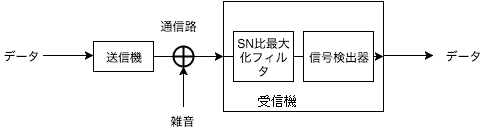
\includegraphics[clip,width=1.05\hsize]{img/matched_filter.png}
\caption{送受信モデルと整合フィルタ}\label{fig:matched_filter}
\end{figure}


\begin{figure}[p]\centering
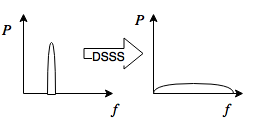
\includegraphics[clip,width=1.05\hsize]{img/DS.png}
\caption{スペクトル拡散によるパルス圧縮}\label{fig:DS}
\end{figure}


\subsection{チャープ信号}

周波数を時間に比例して変化させた波をチャープ信号(Chirp Signal)という.
波形を図\ref{fig:chirpsig}に示し,スぺクトログラムを図\ref{fig:chirpsig2}に示す.
チャープ信号は線形周波数変調(LFM: Linear Frequency Modulated)信号とも呼ばれる.
また,インパルス応答測定の分野においては時間引き伸ばしパルス(TSP: Time Stretched Pulse)とも呼ばれる\cite{Aoshima},.
チャープ信号は,方形パルスを周波数方向へ掃引することで,図\ref{fig:chirppulse_amb}に示すように,
通常パルスと同じ電力で時間方向の精度を向上させることができる(図\ref{fig:chirppulse_amb}).
チャープ信号は受信波形と送信波形との相互相関を求めることにより,
通常の反射波形に変換された信号が得られる.
チャープ信号によるパルス圧縮は,
相関処理により信号を検出するので,
通常のパルス型の音源に比べて
雑音の影響を受けにくいという利点がある.
また,パルス型の音源に比べ瞬間のエネルギーは小さいが,
送波時間を長くすることにより,
相関後のエネルギーを通常パルスよりも大きくすることができるというパルス圧縮の効果が得られる.
チャープ信号はレーダーやソーナー,インパルス応答の測定に利用されている.


\begin{figure}[p]\centering
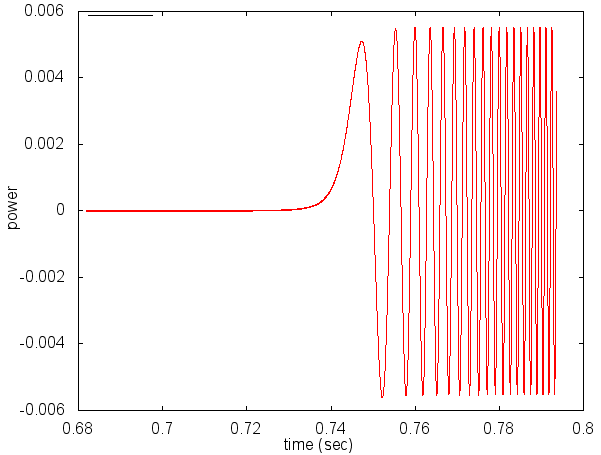
\includegraphics[clip,width=1.0\hsize]{img/chirp.png}
\caption{チャープ信号波形}\label{fig:chirpsig}
\end{figure}

\begin{figure}[p]\centering

\includegraphics[clip,width=0.7\hsize]{img/chirp_spectogram.png}\\
\caption{チャープ信号スぺクトログラム}\label{fig:chirpsig2}
\end{figure}


\begin{figure}[p]\centering
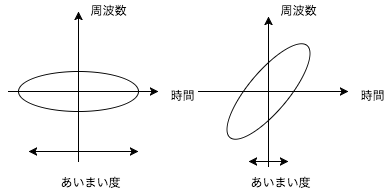
\includegraphics[clip,width=0.9\hsize]{img/aimai.png}\\
通常パルス~ ~ ~ ~ ~ ~ ~ ~ ~ ~ ~ Chirpパルス
\caption{通常パルスとチャープパルスによる曖昧度の比較}\label{fig:chirppulse_amb}
\end{figure}



\subsection{PSK信号}
チャープ信号はドップラー効果の周波数ずれに対してパルス位置が変わるだけで,サイドローブは劣化しにくい.
しかし,継続時間の長いチャープ信号は曖昧度関数のピーク周辺のサイドローブが大きくなるため,
非常に遠距離間での信号検出や,雑音が大きな環境間での微弱な信号検出には,
継続時間を伸ばしても性能が劣化しにくいM系列符号やそれを応用した符号系列を用いた
直接スペクトル拡散(DSSS: direct sequence spread spectrum)が用いられる.
直接スペクトル拡散変調は,位相偏移変調方式(PSK:Phase-shift keying)により,ビット系列で正弦波を変調する.
特に,正弦波の位相を0と $\pi$ に変化させ,それぞれ1と-1を割り当てる場合,
2値符号変調方式(BPSK:Binary Phase-shift keying)という.
PSC信号では,チャープ信号と同じく通常パルスと比べ.
パルス幅を長く保ったまま時間分解能を上げることができる.
また,ビット系列の選び方によって相関処理後のサイドローブが変化する.
サイドローブを抑える系列として,バーカー符号とM系列符号がある.
PSK信号とチャープ信号とを比較すると,
PSK信号は対象物が移動してドップラー効果が生じるような場合には,サイドローブが劣化しやすく,
また,非線形な歪みを生じることがある.

\begin{figure}[p]\centering
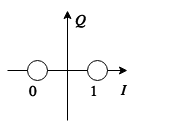
\includegraphics[clip,width=0.27\hsize]{img/chirp_qi.png}
\caption{BPSK信号空間ダイヤグラム}\label{fig:chirpqi}
\end{figure}

\subsection{バーカー符号}
バーカー符号(Barker code)(図\ref{fig:barkercode})は直接スペクトル拡散変調によるパルス圧縮に用いられる符号系列の一種である.
同期点以外での自己相関関数の絶対値の最大が$1/N$となる長さ$N$の有限長系列で,長さ13まで存在し,
相関特性が長さ13の場合,ピークが13倍,サイドローブが1/13倍となるような,
ディラックの$\delta$関数に近い理想的な相関特性を持つ.

バーカー符号はサイドローブをできるだけ小さくするような符号列であり,
サイドローブがすべて $1/N^2$ になる系列である.
バーカー符号は $N=13$ までしか知られていないが,
さらにパルス圧縮して時間分解能を上げたい時は,M系列符号を使う.
バーカー符号はレーダーやソナー,ロケットのトランスポンダ\cite{高野忠00}など利用されている.

\begin{figure}[p]\centering
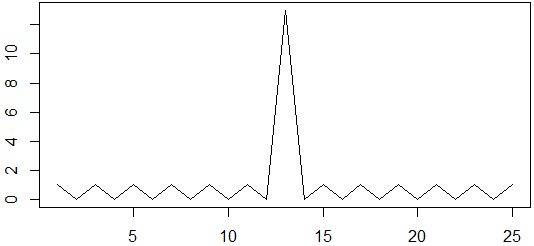
\includegraphics[clip,width=0.9\hsize]{img/barkercode.png}
\caption{Barker符号(13列)の自己相関}\label{fig:barkercode}
\end{figure}

\begin{table}[p]\centering
  \caption{バーカー符号の種類とサイドローブレベル}
  \label{tab:barker}
  \begin{tabular}{l|ccc}
    \hline
    長さ N & 系列 $\{q_n\}$ & サイドローブ[dB] \\
    \hline
    2  & 1,-1 | 1,1                   & -6.0 \\
    3  & 1,1,-1 | 1,1                 & -9.5 \\
    4  & 1,1,-1,1 | 1,1,1,-1          & -12.0 \\
    5  & 1,1,1,-1,1                    & -14.0 \\
    7  & 1,1,1,-1,-1,1,-1              & -16.9 \\
    11 & 1,1,1,-1,-1,-1,1,-1,-1,1,-1   & -20.8 \\
    13 & 1,1,1,1,1,-1,-1,1,1,-1,1,-1,1 & -22.3 \\
    \hline
  \end{tabular}
\end{table}



\subsection{M系列符号}
最大周期シフトレジスタ(Maximum length shift register)系列は,M系列とも呼ばれ,
線形帰還シフトレジスタ(LFSR: Linear feedback shift register)を使って生成される擬似雑音(PN)系列の一種である.
LFSRとは,図\ref{fig:LFSR}のような排他的論理和による帰還タップを持つシフトレジスタである.
バーカー符号が有限の符号系列であるのに対して,M系列符号は有限の符号系列が周期的に繰り返される.
M系列は.LFSRに全てゼロ以外の初期値を与えることにより生成される周期系列のうち,
周期 N が最大となるものである.
1周期中に全ゼロ以外の全ての k ビットパターンが必ず1回出て来くるので,$N=2^k-1$ となる.
このような系列はLFSRの帰還結線の位置がある限られた組み合わせを満たすときのみ生成され,
それ以外の場合は周期のより短い系列となる.
M系列の系列の長さNが十分に長いとき,
曖昧度関数のサイドローブの最大値は $1/N$ となる\ref{fig:mseqautocorrel}.
M系列符号は系列を長くしてもサイドローブを抑えることができるという特徴から,
微弱信号の検出が必要とされる深宇宙探査機との通信\cite{dsn}や海洋音響トモグラフィ\cite{tomography}などに使われている.
また,初期値が異なるM系列どうしの相互相関は直交しピークを持たないという性質から,
通信分野において符号分割多元接続(CDMA:Code Division Multiple Access)に利用される.

\begin{figure}[p]\centering
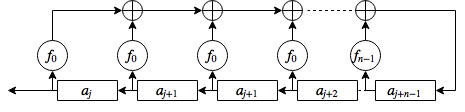
\includegraphics[clip,width=0.9\hsize]{img/M-sequence.png}
\caption{LFSRのブロック線図}\label{fig:LFSR}
\end{figure}


\begin{figure}[p]\centering
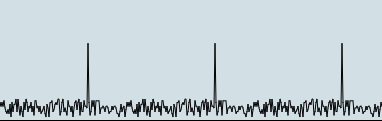
\includegraphics[clip,width=0.9\hsize]{img/mseq_autocorrel.png}
\caption{M系列をBPSK変調した波形の自己相関}\label{fig:mseqautocorrel}
\end{figure}


\section{本研究のスタンス}

以上をまとめると,
スマートデバイスを用いた情報提供システムには,個人向けの研究が目立つ.
また,複数端末を用いてマイクロホンアレイを構築する研究は存在するが,複数端末を用いてのスピーカアレイを構築する手法は比較的未開拓分野と言える.
そして,複数のスマートデバイスを用いて実空間内の複数の人間に働きかける,という本研究のシステムは,
今後さらに生活空間にスマートデバイスが普及することを考えると,
パラコミュニケーションを実現する手段としても重要であると言える.


%\section{菌類とは}
%\section{細菌類とは}
%\section{納豆菌とは}
%\section{納豆菌の既知の効能}
%\section{本研究のスタンス}
